\let\negmedspace\undefined
\let\negthickspace\undefined

\documentclass[journal,12pt,onecolumn]{IEEEtran}
%\documentclass[journal,12pt,twocolumn]{IEEEtran}
%
\usepackage{setspace}
\usepackage{gensymb}
%\doublespacing
\singlespacing

%\usepackage{graphicx}
%\usepackage{amssymb}
%\usepackage{relsize}
\usepackage[cmex10]{amsmath}
%\usepackage{amsthm}
%\interdisplaylinepenalty=2500
%\savesymbol{iint}
%\usepackage{txfonts}
%\restoresymbol{TXF}{iint}
%\usepackage{wasysym}
\usepackage{amsthm}
\usepackage{mathrsfs}
\usepackage{txfonts}
\usepackage{stfloats}
\usepackage{cite}
\usepackage{cases}
\usepackage{subfig}
\usepackage[table]{xcolor}
%\usepackage{xtab}
\usepackage{longtable}
\usepackage{multirow}
%\usepackage{algorithm}
%\usepackage{algpseudocode}
\usepackage{enumitem}
\usepackage{mathtools}
\usepackage{tikz}
\usepackage{circuitikz}
\usepackage{verbatim}
\usepackage{hyperref}
%\usepackage{stmaryrd}
\usepackage{tkz-euclide} % loads  TikZ and tkz-base
%\usetkzobj{all}
\usepackage{listings}
\usepackage{color}                                            %%
\usepackage{array}                                            %%
\usepackage{longtable}                                        %%
\usepackage{calc}                                             %%
\usepackage{multirow}                                         %%
\usepackage{hhline}                                           %%
\usepackage{ifthen}                                           %%
%optionally (for landscape tables embedded in another document): %%
\usepackage{lscape}     
\usepackage{multicol}
\usepackage{chngcntr}
\usepackage{iftex}
%\usepackage[latin9]{inputenc}
\usepackage{geometry}
\usepackage{bm}
%\geometry{verbose,tmargin=2cm,bmargin=3cm,lmargin=1.8cm,rmargin=1.5cm,headheight=2cm,headsep=2cm,footskip=3cm}
\usepackage{array}
\newcolumntype{L}[1]{>{\raggedright\let\newline\\\arraybackslash\hspace{0pt}}m{#1}}
\newcolumntype{C}[1]{>{\centering\let\newline\\\arraybackslash\hspace{0pt}}m{#1}}
\newcolumntype{R}[1]{>{\raggedleft\let\newline\\\arraybackslash\hspace{0pt}}m{#1}}

%\usepackage{graphicx}
%\usepackage{setspace}
%\usepackage{parskip}

\def \hsp {\hspace{3mm}}

\makeatletter

\providecommand{\tabularnewline}{\\}



\makeatother
\ifxetex
\usepackage[T1]{fontenc}
\usepackage{fontspec}
%\setmainfont[ Path = fonts/]{Sanskrit_2003.ttf}
\newfontfamily\nakulafont[Script=Devanagari,AutoFakeBold=2,Path = fonts/]{Nakula}
%\newfontfamily\liberationfont{Liberation Sans Narrow}
%\newfontfamily\liberationsansfont{Liberation Sans}
\fi
\usepackage{tikz}
\usepackage{xcolor}
%\usepackage{enumerate}

%\usepackage{wasysym}
%\newcounter{MYtempeqncnt}
\DeclareMathOperator*{\Res}{Res}
%\renewcommand{\baselinestretch}{2}
\renewcommand\thesection{\arabic{section}}
\renewcommand\thesubsection{\thesection.\arabic{subsection}}
\renewcommand\thesubsubsection{\thesubsection.\arabic{subsubsection}}

\renewcommand\thesectiondis{\arabic{section}}
\renewcommand\thesubsectiondis{\thesectiondis.\arabic{subsection}}
\renewcommand\thesubsubsectiondis{\thesubsectiondis.\arabic{subsubsection}}

% correct bad hyphenation here
\hyphenation{op-tical net-works semi-conduc-tor}
\def\inputGnumericTable{}                                 %%

\lstset{
	language=tex,
	frame=single, 
	breaklines=true
}

%\begin{document}
%


\newtheorem{theorem}{Theorem}[section]
\newtheorem{problem}{Problem}
\newtheorem{proposition}{Proposition}[section]
\newtheorem{lemma}{Lemma}[section]
\newtheorem{corollary}[theorem]{Corollary}
\newtheorem{example}{Example}[section]
\newtheorem{definition}[problem]{Definition}
%\newtheorem{thm}{Theorem}[section] 
%\newtheorem{defn}[thm]{Definition}
%\newtheorem{algorithm}{Algorithm}[section]
%\newtheorem{cor}{Corollary}
\newcommand{\BEQA}{\begin{eqnarray}}
	\newcommand{\EEQA}{\end{eqnarray}}
\newcommand{\define}{\stackrel{\triangle}{=}}
\bibliographystyle{IEEEtran}
%\bibliographystyle{ieeetr}
\providecommand{\mbf}{\mathbf}
\providecommand{\pr}[1]{\ensuremath{\Pr\left(#1\right)}}
\providecommand{\qfunc}[1]{\ensuremath{Q\left(#1\right)}}
\providecommand{\sbrak}[1]{\ensuremath{{}\left[#1\right]}}
\providecommand{\lsbrak}[1]{\ensuremath{{}\left[#1\right.}}
\providecommand{\rsbrak}[1]{\ensuremath{{}\left.#1\right]}}
\providecommand{\brak}[1]{\ensuremath{\left(#1\right)}}
\providecommand{\lbrak}[1]{\ensuremath{\left(#1\right.}}
\providecommand{\rbrak}[1]{\ensuremath{\left.#1\right)}}
\providecommand{\cbrak}[1]{\ensuremath{\left\{#1\right\}}}
\providecommand{\lcbrak}[1]{\ensuremath{\left\{#1\right.}}
\providecommand{\rcbrak}[1]{\ensuremath{\left.#1\right\}}}
\theoremstyle{remark}
\newtheorem{rem}{Remark}
\newcommand{\sgn}{\mathop{\mathrm{sgn}}}
\providecommand{\abs}[1]{\left\vert#1\right\vert}
\providecommand{\res}[1]{\Res\displaylimits_{#1}} 
\providecommand{\norm}[1]{\left\lVert#1\right\rVert}
%\providecommand{\norm}[1]{\lVert#1\rVert}
\providecommand{\mtx}[1]{\mathbf{#1}}
\providecommand{\mean}[1]{E\left[ #1 \right]}
\providecommand{\fourier}{\overset{\mathcal{F}}{ \rightleftharpoons}}
%\providecommand{\hilbert}{\overset{\mathcal{H}}{ \rightleftharpoons}}
%\providecommand{\system}{\overset{\mathcal{H}}{ \longleftrightarrow}}
\providecommand{\system}[1]{\overset{\mathcal{#1}}{ \longleftrightarrow}}
\providecommand{\gauss}[2]{\mathcal{N}\ensuremath{\left(#1,#2\right)}}
%
%\newcommand{\solution}[2]{\textbf{Solution:}{#1}}
\newcommand{\solution}{\noindent \textbf{Solution: }}
\newcommand{\cosec}{\,\text{cosec}\,}
\newcommand{\sinc}{\,\text{sinc}\,}
\newcommand{\rect}{\,\text{rect}\,}
\providecommand{\dec}[2]{\ensuremath{\overset{#1}{\underset{#2}{\gtrless}}}}
\newcommand{\myvec}[1]{\ensuremath{\begin{pmatrix}#1\end{pmatrix}}}
\newcommand{\mydet}[1]{\ensuremath{\begin{vmatrix}#1\end{vmatrix}}}
\newcommand*{\permcomb}[4][0mu]{{{}^{#3}\mkern#1#2_{#4}}}
\newcommand*{\perm}[1][-3mu]{\permcomb[#1]{P}}
\newcommand*{\comb}[1][-1mu]{\permcomb[#1]{C}}
%\numberwithin{equation}{section}
\numberwithin{equation}{section}
%\numberwithin{problem}{section}
%\numberwithin{definition}{section}
\makeatletter
\@addtoreset{figure}{problem}
\makeatother
%\let\StandardTheFigure\thefigure
\let\vec\mathbf
%\renewcommand{\thefigure}{\theproblem.\arabic{figure}}
\renewcommand{\thefigure}{\arabic{section}.\arabic{figure}}
%\setlist[enumerate,1]{before=\renewcommand\theequation{\theenumi.\arabic{equation}}
	%\counterwithin{equation}{enumi}
	%\renewcommand{\theequation}{\arabic{subsection}.\arabic{equation}}
\let\StandardTheFigure\thefigure
	\vspace{3cm}
	%\usepackage{babel}
	\begin{document}
		\title{XGBoost}
		\author{ Mannem Charan AI21BTECH11019}
		 \maketitle
		\begin{abstract}
			This report consists of my basic understanding of one of the popular Ml methods "XGBoost".
		\end{abstract}
		\section{XGBoost}
		  XGBoost is a boosting algorithm which comes under ensemble learning where the decision trees $\brak{\text{weak learners}}$ are combined sequentially to predict the output of the task.It is also known as eXtreme gradient boosting and it is a modification of classical gradient boosting technique.Same as in gradient boost , XGBoost creates decision trees of residual at each step and uses it for prediction.But in doing so it uses something known as "Similarity scores" by which we can get access to new features like pruning trees and regularization.Now we will see Xgboost in action using a dataset as an example.
		\section{Understanding XGBoost}
		  Consider the dataset given below ,\\
		  \rowcolors{2}{gray!10}{gray!40}
		   \begin{tabular}{ccc}
	              Years Of Experience & Gap & Annual Salary$\brak{100k}$ \\
			   \hline 
			 1 & No & 4 \\
			 1.5 & Yes & 4 \\
			 2.5 & Yes & 5.5 \\
			  3 & Yes & 7 \\
			  5 & No & 7.5 \\
			   6 & NO & 8 \\
		    \end{tabular}
	Here the target attribute is "Annual Salary$\brak{100k}$" and to predict that we have two features in our disposal , "Years of Experience" and "Gap".So to start the algorithm, first we need a base learner to make the first prediction.There is no correct way of doing it but in general we will take average of salary as the first prediction.\\
	\begin{enumerate}
         \item Then 
		 \begin{align}
			 F_{0} &= \frac{4 + 4 + 5.5 + 7 + 7.5 + 8}{6}\\
			       &= 6\brak{100K}
		 \end{align}
		Here we are indicating the prediction of base learner as $F_{0}$to make it analagous to what we did in GBM.
	 \item After the first step we will find the pseudo residual values,which is the measure of error due to our first prediction.
		 \begin{align}
			 Pseudo Residual &= observed_i - predicted_i
		 \end{align}
			We are calling it as pseudo residual since if the cost function has fraction $\frac{1}{2}$ then the cost function is similar to that of linear regression where we call the error as "residuals" but often the constant term multiplying may not be $\frac{1}{2}$ that is the reason why we are calling it as "pseudo residuals".\\
	So now our new dataset will be,\\
	   \rowcolors{2}{gray!10}{gray!40}
	     \begin{tabular}{cccc}
	       Years of Experience & Gap & Annual Salary$\brak{100k}$ & Pseudo Residuals \\
		     \hline
		     1 & No & 4 & -2 \\
		     1.5 & Yes & 4 & -2 \\
		     2.5 & Yes & 5.5 & -0.5 \\
		     3 & Yes & 7 & 1 \\ 
		     5 & No & 7.5 & 1.5 \\
		     6 & No & 8  & 2 \\
	      \end{tabular}
         \item In this step, we will construct a DT which predict the residuals.XGBoost follows an unique way doing it, it will first construct a leaf of residuals.And we will calculate similarity/quality score of the leaf using the below formula.
		 \begin{align}
			 Similarity Score &= \frac{\brak{\text{Sum of Residuals}}^2}{No. of Residuals + \lambda}
	         \end{align}
			where $\lambda$ is regularization parameter.\\
		Now if we are doing classification, the similarity score will be
		 \begin{align}
			 Similarity Score &= \frac{\brak{\text{Sum of Residuals}}^2}{\sum_ip_i\brak{1-p_i} + \lambda}\label{classification}
	         \end{align}
			where $p_i$ is the predicted probability of the  $i^{th}$ residual in the leaf.\\
	In this case the similarity score of the leaf is ,
			\begin{align}
				Similarity score &= \frac{\brak{-2 + -2 + -0.5 + 1 + 1.5 + 2}^2}{6 + \lambda} \\
						 &= \frac{0}{6 + \lambda}\\
						 &= 0
			\end{align}
	The similarity score is the measure of how similar are residuals in a leaf.Now we will split the leaf in say that the chidrens have more similarity scores than the leaf we actually took. For that we will take Exp <2.75 as decsion maker. 
			\begin{figure}[ht!]
			 \centering
			 \includegraphics[width = 10cm]{first_split.png}
			 \caption{First Split}
			 \label{1}
			\end{figure}
	Now we will calculate similarity scores of left and right branches with $\lambda = 0$,
			\begin{align}
			 S_{L} &= \frac{\brak{-2 + -2 + -0.5}^2}{3 + \lambda}\\
			       &= \frac{\brak{-4.5}^2}{3 + 0}\\
			       &= 6.75\\
			 S_{R} &= \frac{\brak{1 + 1.5 + 2}^2}{3 + \lambda}\\
			       &= \frac{\brak{4.5}^2}{3 + 0}\\
			       &= 6.75
		        \end{align}
           Then we will calculate the \textbf{Gain} for this split,
			\begin{align}
				Gain &= S_{L} + S_{R}- S_{\text{Root}} \\
				     &= 6.75 + 6.75 - 0 \\
				     &= 13.5
		        \end{align}
		And I will assure you that it is the best split as we are able to "cluster" the similar residuals into different groups.\\
		Then we will again split the DT with Gap as the parameter, 
			 \begin{align}
				 S_{L} &= \frac{\brak{-2-0.5}^2}{2 + \lambda}\\
				       &= \frac{6.25}{2 + 0}\\
				       &= 3.125 \\
				 S_{R} &= \frac{4}{1+ 0} \\
				       &= 4
                         \end{align}
                 Then Gain in this split will be,
		         \begin{align}
				 Gain &= S_{L} + S_{R} - S_{Root} \\
				      &= 3.125 + 4 - 6.75 \\
				      &= 0.375
		         \end{align}
		So the final DT will be as in $\ref{2}$,
		      \begin{figure}
			\centering
			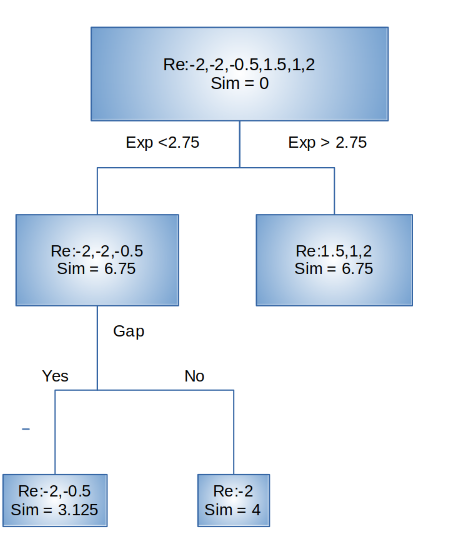
\includegraphics[width = 10cm]{Second_split.png}
			\caption{Residual tree}
			\label{2}
		      \end{figure}
		  Now before going to predict the output of each leaf node we will first understand what is the role of $\lambda$.In XGBoost to prune the branches we will check whether the value $\text{Gain} - \gamma$ is greater or less than 0.This $\gamma$ is user-defined so it is a tuneable parameter in the model.Now we can clearly say that when $\lambda > 0$ the similarity scores will be lesser which make the overall \textbf{Gain} to be smaller than the older value.So depending on $\lambda$ we will prune the trees using the following heuristic,
		   \begin{align}
			   Gain - \gamma &= \begin{cases}
				               >0 &, \text{then do not prune} \\
					       < 0 &, \text{then prune}
					     \end{cases}
                    \end{align}
		    In Classification, using the equation mention in $\eqref{classification}$ we will find the gain in each split and using that we will prune the branches\textbf{and also} there is something known as "\textbf{Cover}" which is nothing but the replacement for number of residuals in denominator of similarity score in classification i.e.,
		    \begin{align}
			    Cover &= \sum_ip_i\brak{1-p_i}
		    \end{align}
		    Now the deal here is the cover should have a minimum value of 1, if it not the case we will simply remove that leaf node.This term analagous to the no. of residuals term in regression.\\ 
		   And the last thing is if you remember when we started creating the DT we said we take leaf where it later splits into branches then we are again refering it as root. The thing is, depending on choice of parameter $\gamma$ and $\lambda$ it may happen that we will prune all the branches and left with the leaf itself.So we kinda start creating tree with our output/leaf node as the root itself.
	   \item In this step, we will compute the output values of each leaf node.This is similar to what we did in Classical GBM but here we will have extra $\lambda$,
		   \begin{align}
			   Output = \frac{\text{Sum of Residuals}}{\text{Number of Residuals} + \lambda}
		   \end{align}
		   Note that $\lambda$ value is also responsible in shrinking the output value.\\
                   And for the Classification the output will be,
		   \begin{align}
			   Output &= \frac{\text{Sum of Residuals}}{\mathbf{Cover} + \lambda}
		   \end{align}
            In this case, the output value of each leaf node will be as shown in fig $\ref{3}$,
	           \begin{figure}
		     \centering
		     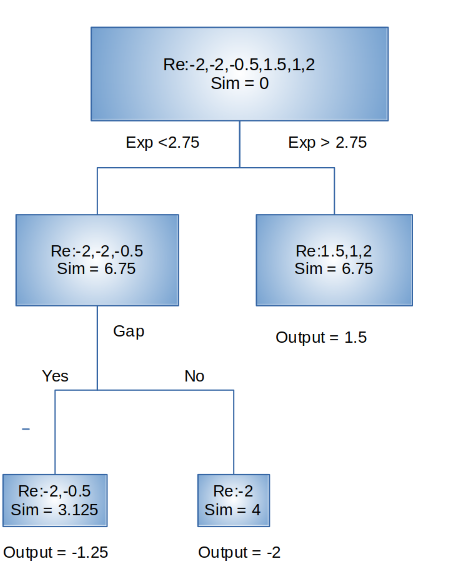
\includegraphics[width = 10cm]{Finaltree.png}
		     \caption{Residual Tree with predicted output}
		     \label{3}
	            \end{figure}
	    \item In final step, we the help of learning rate we will make a new prediction using old prediction and the residual tree.
		    \begin{align}
			    New prediction &= Old prediction + \eta\brak{\text{output from residual trees}}
		    \end{align}
		       where, $\eta$ is the learning rate.\\
		     In this case, we will take $\eta = 0.3$ and using that the new predictions of each input instance $x_i$ will be ,
		       \begin{align}
			       F_{1}\brak{x_1} &= F_{0}\brak{x_1} + 0.3\brak{-2}\nonumber\\
			                       &= 6 - 0.6\nonumber\\
					       &= 5.4 \\
			       F_{1}\brak{x_2} &= F_{0}\brak{x_2} + 0.3\brak{-1.25}\nonumber \\
			                       &= 6 - 0.375\nonumber\\
					       &= 5.625\\
			       F_{1}\brak{x_3} &= F_{0}\brak{x_3} + 0.3\brak{-1.25}\nonumber \\
			                       &= 6 - 0.375\nonumber\\
                                               &= 5.625\\
                               F_{1}\brak{x_4} &= F_{0}\brak{x_4} + 0.3\brak{1.5}\nonumber \\
			                       &= 6 + 0.45\nonumber \\
					       &= 6.45\\
			       F_{1}\brak{x_5} &= 6.45\\
			       F_{1}\brak{x_6} &= 6.45
			\end{align}
		So the new dataset looks like,\\
		\rowcolors{2}{gray!10}{gray!40}
		\begin{tabular}{ccccc}
			Years of Experience & Gap & Annual Salary$\brak{100k}$ & NewPrediction & New Residuals \\
			\hline
			1 & No & 4 &  5.4 & -1.4\\
			1.5 & Yes & 4 & 5.625 & -1.625 \\
			2.5 & Yes & 5.5 & 5.625 & -0.125 \\
			3 & Yes & 7 & 6.45 & 0.55\\ 
			5 & No & 7.5 & 6.45 & 1.05 \\
			6 & No & 8  & 6.45 & 1.55\\
		\end{tabular}
		  \\
	           As you can see we moved in right direction for each input instance and from these assumptions we will construct a new Residual tree and so on.\\
		In Classification we will do things slightly different, we will find the $\log\brak{\text{odds}}$ of the intial predicted probability and add it with thescaled output from the residual tree. Then we will again convert the resulting value into probability.This value will be the new predicted probability.The following is the expression of finding $\log\brak{\text{odds}}$ from the probability $p$ and vice- versa,
		 \begin{align}
			 \log\brak{odds} &= \log\brak{\frac{p}{1-p}}\\
			  p &= \frac{e^{\log\brak{odds}}}{1 + e^{\log\brak{odds}}}
                 \end{align}
              With this we covered most of the concepts behind XGBoost.
   \end{enumerate}
           \section{Advantages of XGboost}
	     Some of the advantages of XGBoost are as follows,
	       \begin{itemize}
		\item Effective with large data sets.
	        \item The model is highly flexible
	        \item It supports regularization
	        \item It doesn't requires normalization
	       \end{itemize}
	     \end{document}



                                                      



